\section{Framing-based Camera Tool (FCT)}
\subsection{Framing Concept}
In traditional animation, keyframes correspond to a point in time, meaning that when the animation reaches this point in time, the values of this particular keyframing are dominating. Usually, this means that in between keyframes some interpolation is happening. 

%This interpolation is per default linear, but can be manipulated in a graph editor. Anything that can be represented by numbers can be manipulated through keyframes.

Since games don't follow a linear structure like a movie, keyframes can't be associated with a point in time, . In this game, the player is able to move freely around within a pre-defined path. FCT is designed with the player's position in mind. Instead of associating keyframes with time, they are associated with positions in the game's world.

%The game is path-based, which means that the player can only walk on a pre-defined path.

To avoid confusion with traditional keyframing, ours have been dubbed \textit{framings}. A framing consists of an \textit{influence point} and a \textit{camera} (see Figure \ref{fig:framingConceptNew}). The camera holds all of the camera features, such as position and rotation of the camera, as well as field of view. The influence point only has a position. When the player's position is the same as an influence point, the associated camera will dominate. This means that the main camera will use the settings of this camera. Moving between influence points causes an interpolation between each associated camera. Additionally, the interpolation can be manipulated in a graph editor.

\begin{figure}[htbp]
\centering
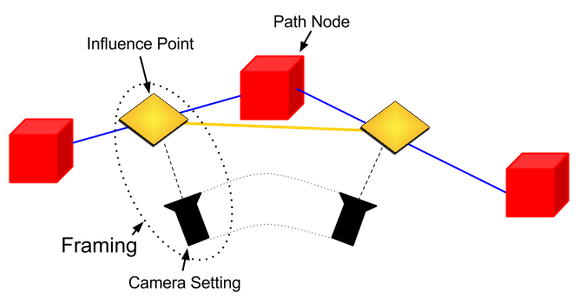
\includegraphics[width=0.4\textwidth]{Pics/Instructions}
\caption{Illustration of the framing concept. A framing consists of an influence point and a camera.}
\label{fig:framingConceptNew}
\end{figure}

\subsection{Path System}
The other programmers on the FEELS team constructed a path-system prior to us making the camera tool. Our tool was dependent on how this system worked for both the interface of our system and the calculations.

The path system consists of connected \textit{pathnodes}, these connections being the \textit{paths}. When the player taps the screen, the closest point to that tap on a path is found and the player character moves along the paths to the selected point. The function for finding this point is what we used to snap influence points to the paths. Making a linear search through the paths for framings (as explained in Section \ref{interpolationChapter}) meant the paths had to log what influence points were on it.

\subsection{Placing an Influence Point}
After a path has been defined, framings can be placed along this path using the mouse. To indicate that an influence point is going to be created, a small diamond-shaped icon appears near the cursor (see Figure \ref{fig:placingInfluencePoint}). This point snaps to the path. Since the player can only work on the path, it is impossible to create an influence point outside of the path. When clicking with the mouse on the path, the system creates a framing. The connection between an influence point and camera is indicated by a small line. The influence point and the camera can be moved and adjusted independently.

Creating a framing while having another framing selected connects the two. This connection is needed for manipulating the interpolation. The interpolation can be adjusted using the built-in graph editor in Unity (see Figure \ref{fig:curve}).

\begin{figure}[htbp]
\centering
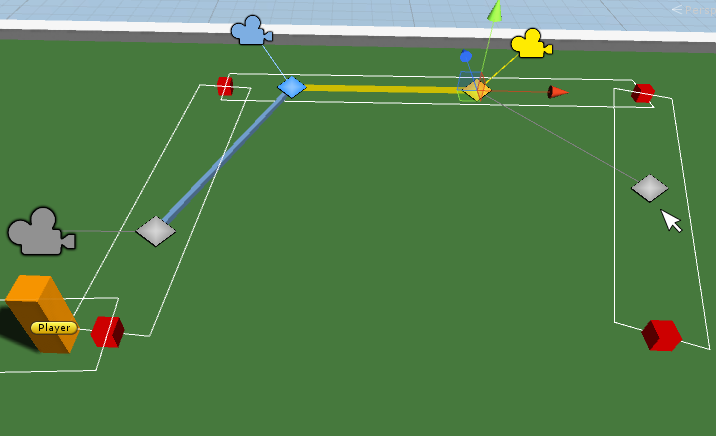
\includegraphics[width=0.45\textwidth]{Pics/placingInfluencePoint}
\caption{You place influence points by holding down the CTRL key and clicking with mouse. These snap to the path defined by the red cubes.}
\label{fig:placingInfluencePoint}
\end{figure}

%Additionally, it is possible to create multiple framings and connect them to each other. This is achieved by selecting an already-created influence point and then clicking to create a new one besides it.

Since the influence point and camera constitutes a framing, the system has been designed so selecting either one selects the framing; hence both provide the same options in the settings window.

\begin{figure}[htbp]
\centering
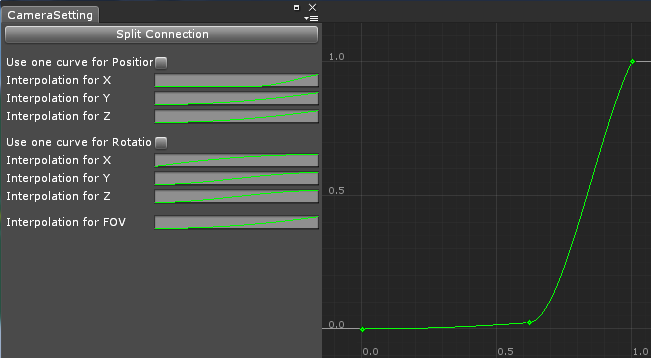
\includegraphics[width=0.45\textwidth]{Pics/curve}
\caption{The graph editor can adjust the interpolation of the position, rotation and field of view.}
\label{fig:curve}
\end{figure}
\subsection{Adjusting a Camera}
%In Maya, there are multiple ways to accomplish the same thing. An example of this is how to adjust a camera in the scene. This can be done by manually adjusting the X, Y and Z position and rotation of the camera; moving it by dragging a handle tool; or, alternatively, by using the the \textit{Look Through Selected} feature \cite{maya_lookThrough}. During the initial observations, it was clear that many of the artists at The Animation Workshop preferred the latter. This concept was translated directly into the camera tool. Using the \textit{be the camera} feature (see Figure \ref{fig:beTheCam}), the artists can place their camera by navigating the scene in Unity with the \textit{Flythrough mode} \cite{unity_flyMode}.

Besides the traditional ways of aligning objects in Unity (either manually changing X, Y and Z coordinates or adjusting an object via handle gizmos), FCT provides three additional ways: \textit{be the camera}, \textit{snapshot} and \textit{aim point}. The first two take advantage of the scene view in Unity where it is possible to control the camera in a similar way as in first-person controlled computer games. This feature is called the \textit{flythrough mode} \cite{unity_flyMode}. When clicking the \textit{be the camera} button, the tool enters a special mode where the active camera object is automatically aligned to the scene view camera. This means that whatever is visible in the scene view will also be visible by the framing camera. The feature will continue to be enabled until the user exits by pressing the \textit{exit the camera} button. Figure \ref{fig:beTheCam} illustrates this concept. \textit{Snapshot} provides a similar feature, but whereas \textit{be the camera} is continuously activated, \textit{snapshot} only happens one time when the button is pressed.

\begin{figure*}[htbp]
\centering
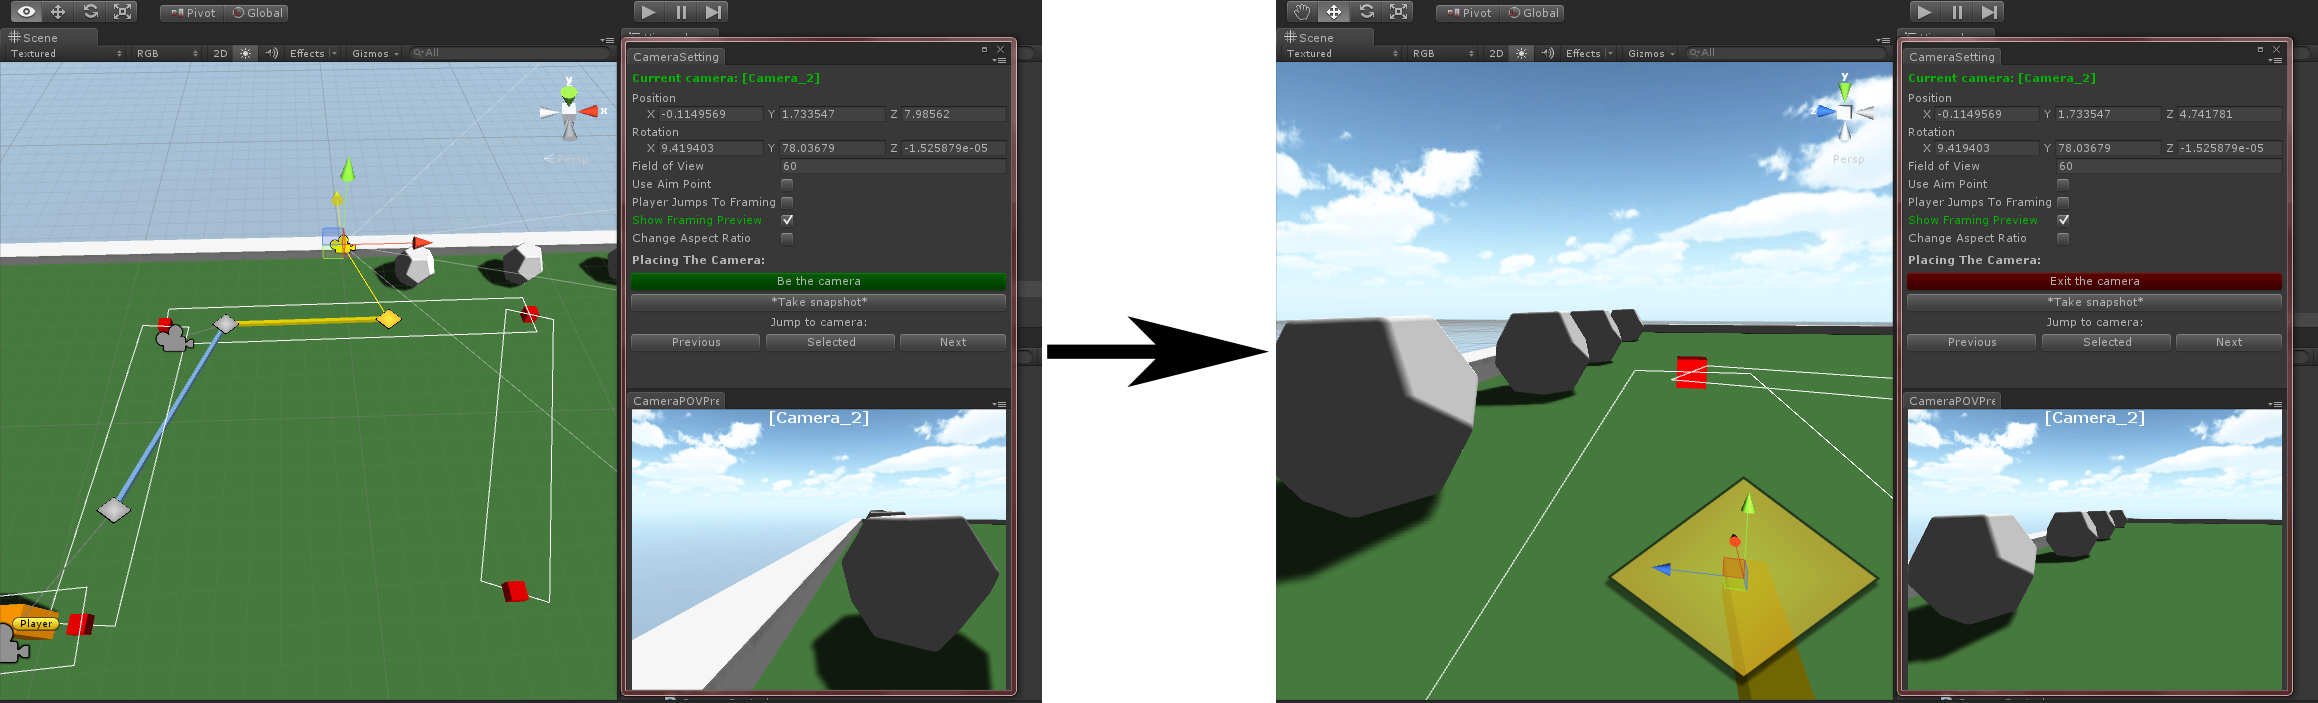
\includegraphics[width=1\textwidth]{Pics/beTheCam}
\caption{Pressing the green button puts the user in a special mode where the selected camera inherits position and orientation data from the scene camera. Notice that only a single rock is visible in the left image. The right image shows how the camera can be moved with the \textit{be the camera} feature to reveal more rocks. The preview image with the [Camera\textunderscore 2] label is how it will look in the actual game.}
\label{fig:beTheCam}
\end{figure*}

A different approach to adjust the camera is by aiming it. This is done with the \textit{aim point}. As the name suggests, the camera will automatically look at this point. This can be used to quickly point at a specific object in the scene, instead of changing the rotation by hand (see Figure \ref{fig:aimPoint}).

\begin{figure}[htbp]
\centering
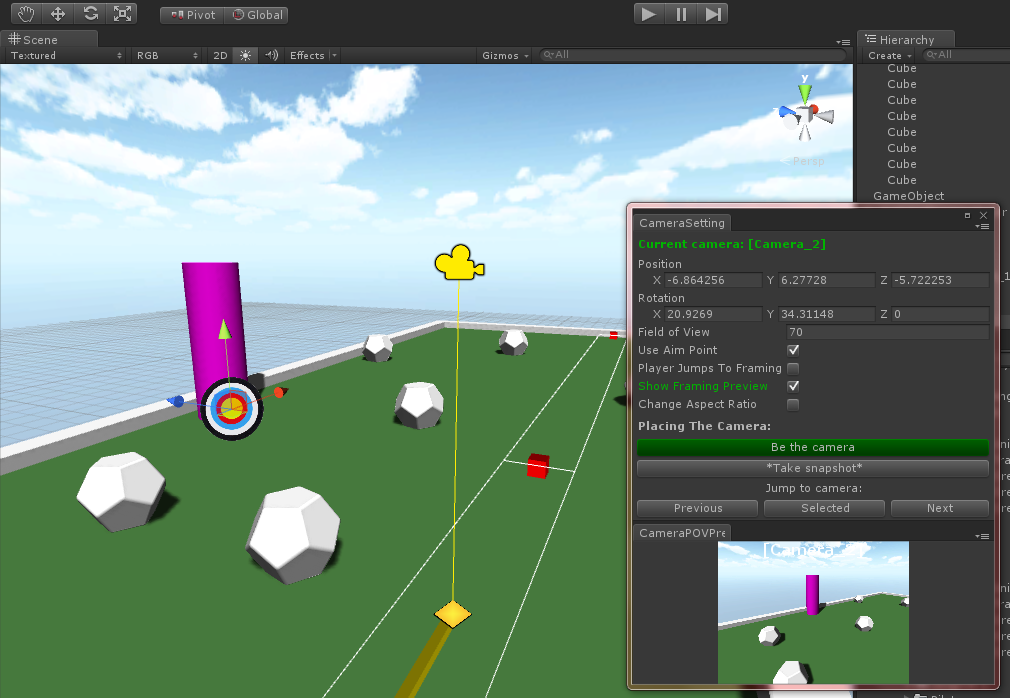
\includegraphics[width=0.4\textwidth]{Pics/aimPoint}
\caption{The aim point (located near the purple cylinder) allows for quick adjustments of the camera.}
\label{fig:aimPoint}
\end{figure}

%It was discovered that none of the artists knew how to use a standard Unity feature that lets the player fly around with the scene camera as if they were playing a first-person game ("Flythrough Mode", \cite{unity_flyMode}). The artist were excited about the discovery of this feature. One artist perceived the standard way of moving around in Unity as confusing, while another stated that the way of moving the camera is exactly like in Maya. After testing this ourselves, we concluded that the movement controls in Maya and Unity are indeed very similar (except for the "Flythrough Mode"), which means that the artists should ideally be comfortable with navigating in either of the applications.

\subsection{Previewing the Interpolations}
FCT provides two ways of previewing the interpolations. One way is to drag the player object around along the path via the \textit{interactive preview}. A different way is to use the \textit{slider preview}. Here, it is possible for the user to select a start framing and end framing and then drag a slider back and forth, changing the interpolation. This provides a quick way to get a feeling of how the camera will interpolate between the framings. Additionally, a "play" button can be pressed to play the interpolation with the actual player velocity (see Figure \ref{fig:slider}).

%The drawback of this method is that you have to manually locate and move the player around in the scene view, which can sometimes be cumbersome.

%An important aspect for the tool was to provide clear feedback.
%A common request from all of the artists were the ability to quickly preview their changes. Instead of having to start the game and navigate the player character to a specific framing, the artists wanted to quickly jump to a specific framing to test out how it feels and looks.

%The artists suggested that they should be able to move the player character around in the editor. Initially, this seemed like a fine way to preview the framings. We did design this feature, but deemed it a bit impractical, since it sometimes would be hard to locate the player character in a big scene. Instead, we took inspiration from Camera Path Animator 3.0 mentioned in Section \ref{relatedWork} by designing an interactive slider. With this feature, the artists are able to choose the start and end framing and interpolate between these. By dragging the slider between those, the artists can quickly get a feel of how the camera movements will look (see Figure \ref{fig:slider}). Alternatively, they can press a "play" button to preview the interpolation and get a feel of the actual player velocity.

\begin{figure}[htbp]
\centering
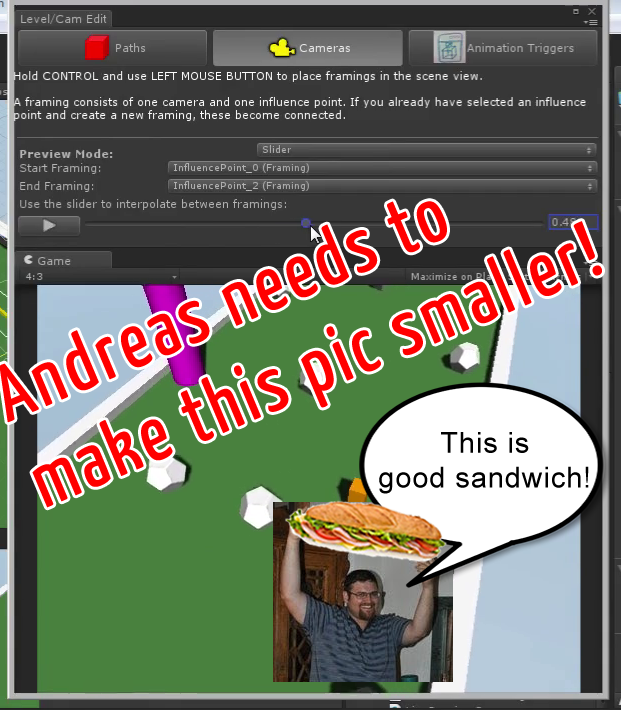
\includegraphics[width=0.45\textwidth]{Pics/slider}
\caption{The slider provides a quick way to preview the framings.}
\label{fig:slider}
\end{figure}

%\subsection{Participatory Design Conclusion}
%It's important to design and iterate with the users' current workflow and mental models in mind. By building on top of their pre-exisiting skills and knowledge, one can ease the learning curve by creating a design that is close to what the users are already familiar with. The users should become co-creators, but you should not forget that \textit{you} are the designer. You should listen to what the users say they want, but even more so try to understand what they really \textit{need} and \textit{why} they need it.